\label{chap:ii}
%%Chap4.tex
%ここでは静的なテキスト集合を対象とした転置インデクスを想定する


本章では本問題に対する転置インデクスの管理・利用について説明する.

遅延評価法はマッチング判定の際に,共通単語を1つも持たないテキストに対してもマッチング判定を行っている.共通単語を1つも持たないとき,Jaccard類似度は0となり類似判定をする必要がない.転置インデクスを用いると共通単語を含むテキストのみを参照することができ,Jaccard類似度が0になるテキストへのマッチング判定を避けることができる.よって遅延評価法に転置インデクスを用いたマッチング判定処理を導入することで類似性判定の処理の高速化を狙う.

\section{データ構造}
マッチング判定はスライディングウィンドウ内のテキストを対象としているので,ユーザ$U$が持つ時刻$T$でのテキスト集合$U_T$は,スライディングウィンドウの大きさ$W$を用いて$U_T=\{u_{T-W+1}, u_{T-W+2}, \cdots u_T\}$と表せる.そしてテキスト$u_T$が持つ単語は,$u_T=\{t_1, t_2, \cdots, t_{|u_T|}\}$と表せる.各テキストはそれぞれが持つ単語によって索引付けされ,単語$t_i$に対するリスト$L_i$は$\langle\mbox{ID}(u_T), f_i\rangle$と表されるテキスト情報を持ち,$\mbox{ID}(u_T)$はテキスト$u_T$が持つテキストID,$f_i$はテキスト$u_T$内の単語$t_i$の出現回数である.$u_T$のハッシュ値を計算し,その値にリスト$L_i$を対応させたハッシュテーブルを転置インデクスとする.

%あるテキスト$Q$に存在する単語を含むテキストをテキスト集合から検索す%る環境を想定し,その環境下での転置インデクスの利用方法を述べる.静%的なテキスト集合に対して転置インデクスを活用することで大規模なデー%タに対する高速な検索が実現できる.
%ここでもテキストは単語集合であるとする.

\section{構築}

静的なテキスト集合を対象とした転置インデクスであれば,テキスト集合の内容は変化せず,転置インデクスを更新する必要はない.しかし,本問題は動的なテキスト集合を扱うため転置インデクスを更新する必要がある.そのため動的なテキスト集合に適した転置インデクスのデータ構造を提案する.
テキストストリームには毎時刻スライディングウィンドウに新しいテキストが到着し,古いテキストが離脱する.このことから単語$t_i$に対応付けられるリスト$L_i$にはキューを用いる.新しいテキストが到着したときには$L_i$の先頭に追加,古いテキストが離脱するときには$L_i$の末尾からテキストを削除とすることで管理コストを抑えつつ動的なテキスト集合に対応した転置インデクスを管理できると考える.

よって転置インデクスの単語$t_i$に対するリスト$L_i$には先頭に近いほど新しいテキストが格納されることになる.転置インデクスの構成を図\ref{fig:ii}に示す.
\begin{figure}[H]
    \centering
    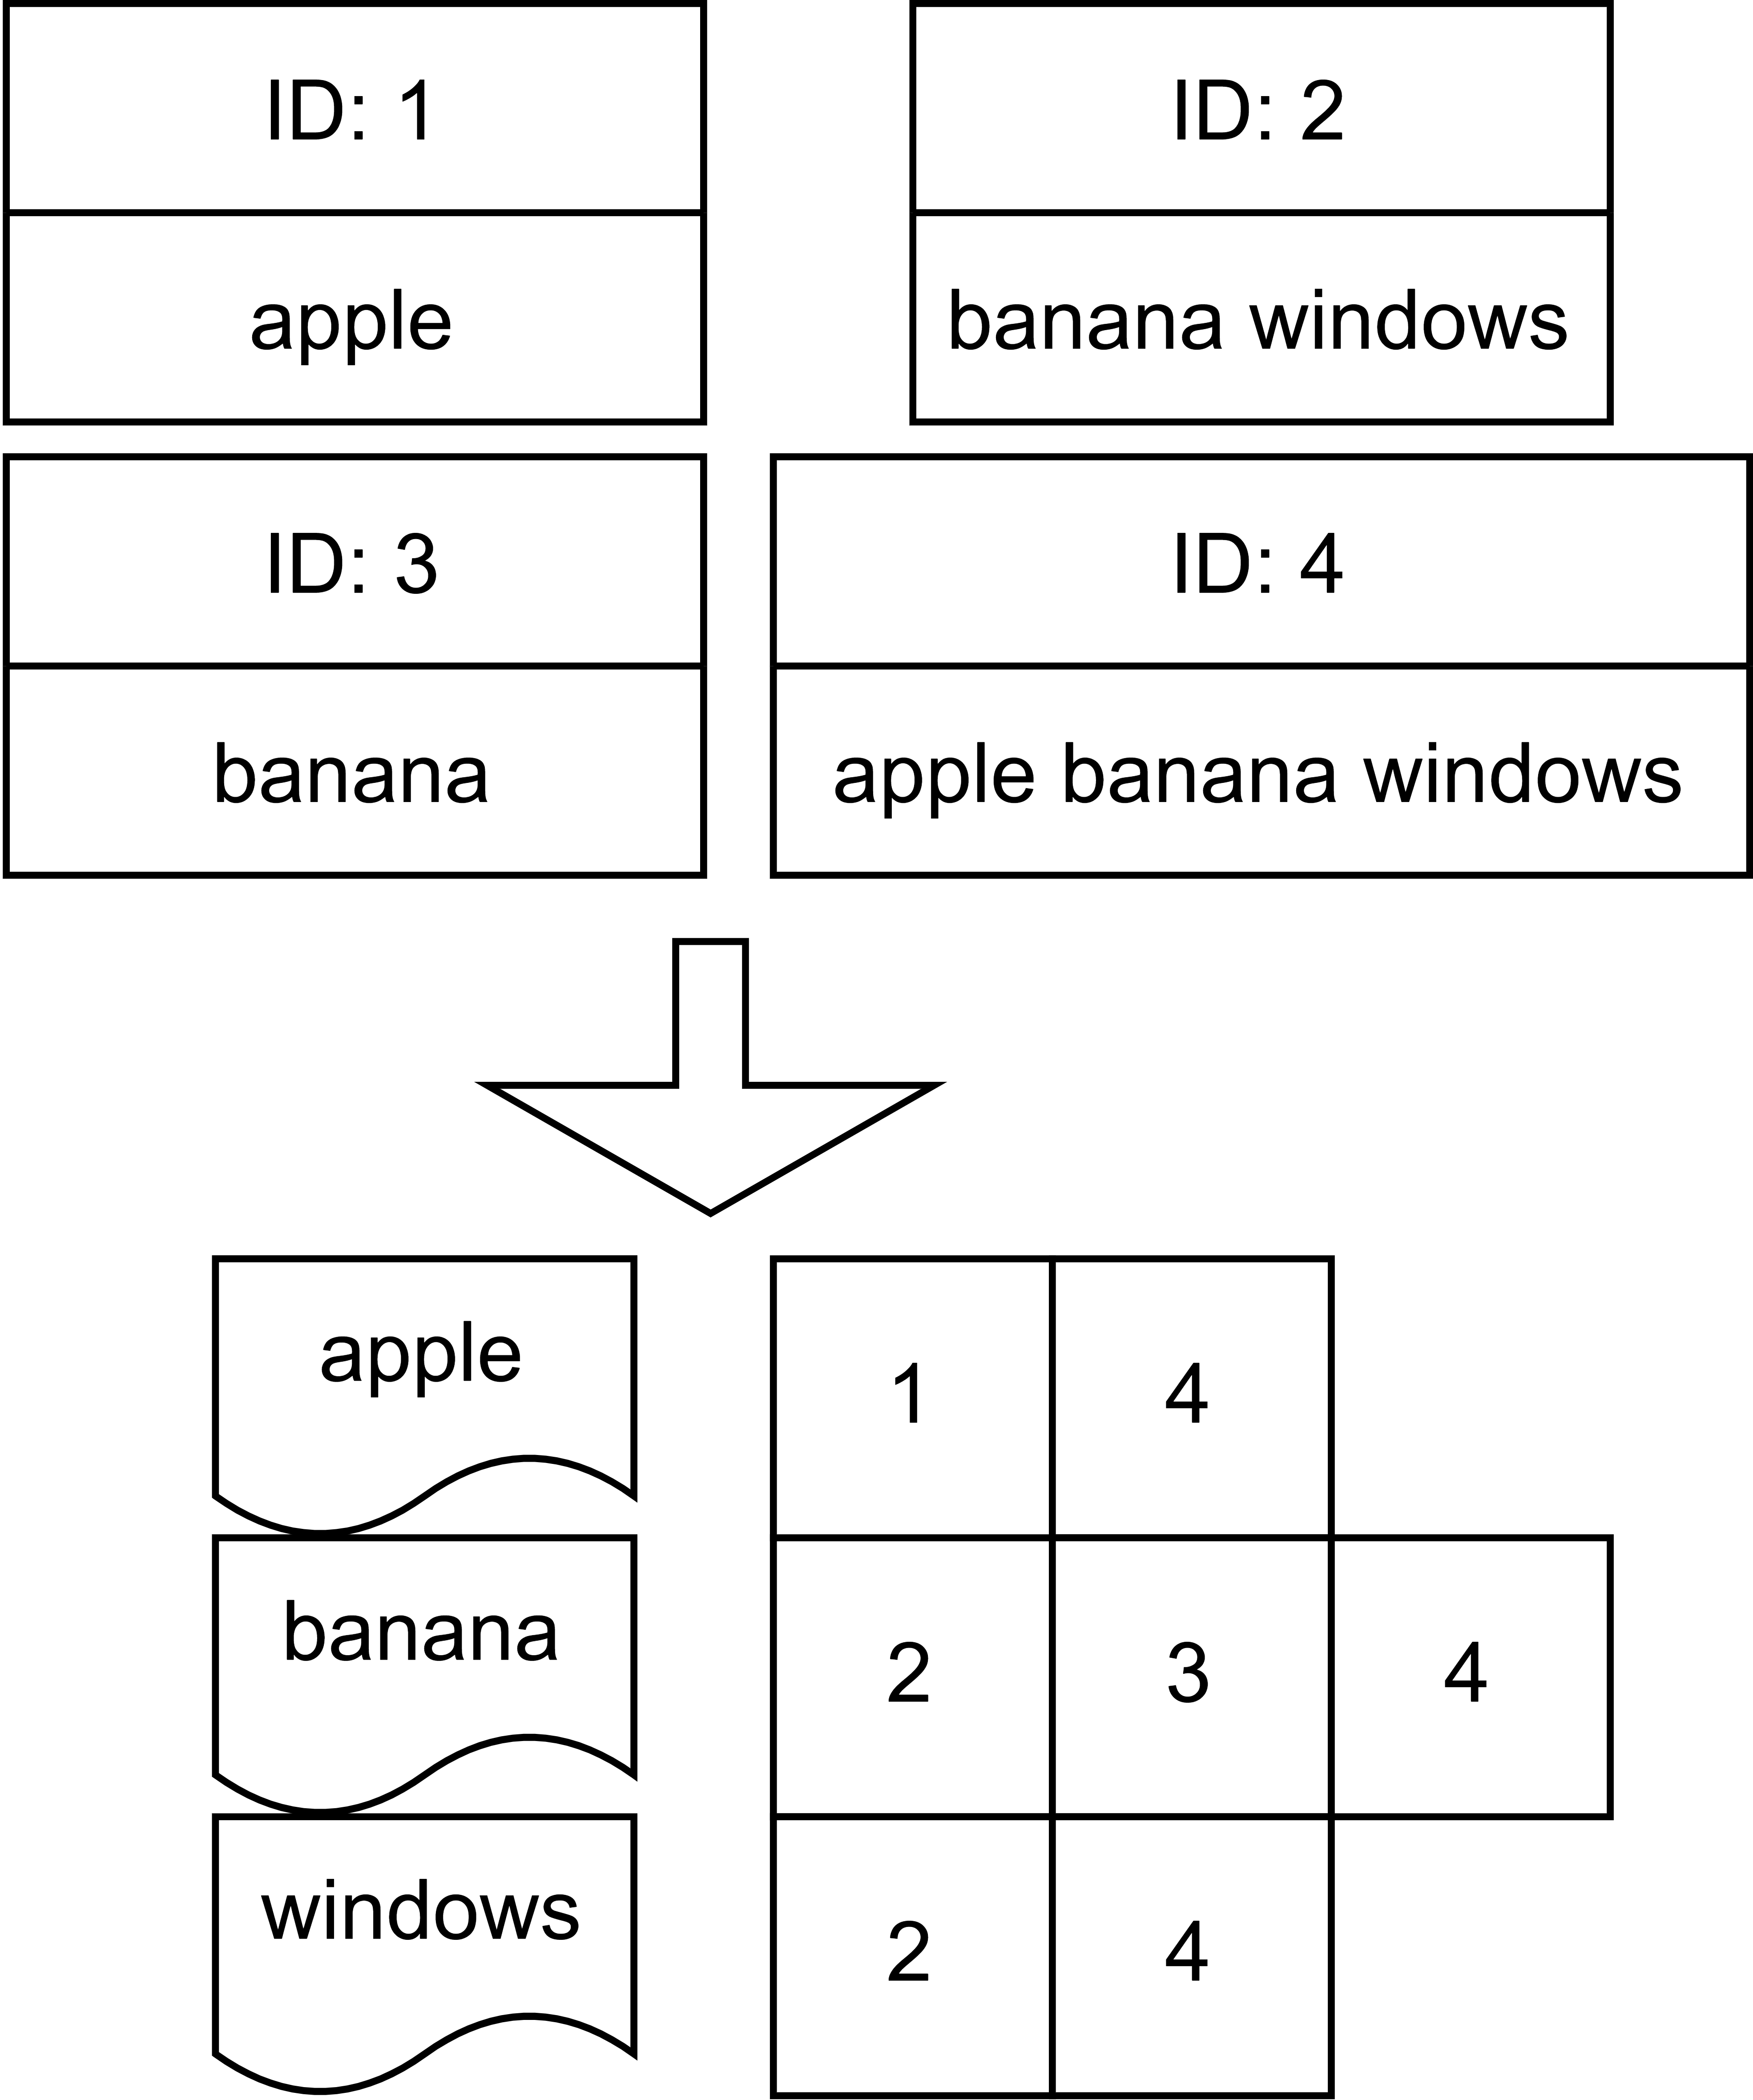
\includegraphics[width=8.7cm]{img/ii.png}
    \caption{転置インデクスの構成}
    \label{fig:ii}
\end{figure}

\section{利用}

テキスト集合$U_T$とテキスト集合$V_T$のテキストについて極大マッチングを求めることを考える.テキスト集合$V_T$に対して転置インデクス$ii_{V_T}$が構築されているとする.
まず,テキスト集合$U_T$からテキスト$u_T$を取り出す.テキスト$u_T$が持つ単語$t_1, t_2, \cdots, t_{|u_T|}$に対応するリストを$ii_{V_T}$から取得するが,ここで取得したリストを用いてテキストを参照する方法が2つ存在する.
\begin{itemize}
    \item TAAT (Term-At-A-Time)
    \begin{description}
        \setlength{\leftskip}{0.25cm}
        \item 単語単位で処理を行う.
        \begin{enumerate}[手順 1]
        \setlength{\leftskip}{0.7cm}
            \item アキュムレータ($acc$)を用意する.
            \item \label{taat:rep} $u_T$から単語$t_1$を取り出し,対応するリストに含まれる全てのテキスト情報を$acc$に追加する
            \item 手順\ref{taat:rep}をすべての単語に対して行う.
            \item $acc$が$u_T$に含まれるテキストを1つでも含むテキストの情報である.
        \end{enumerate}
        アキュムレータに追加されていくテキスト情報は$u_T$から取り出す単語の順番に依存しており,追加される順番に一貫性はない.TAATの手順を図\ref{fig:TAAT}に示す.
    \end{description}
    
    \begin{figure}[H]
        \centering
        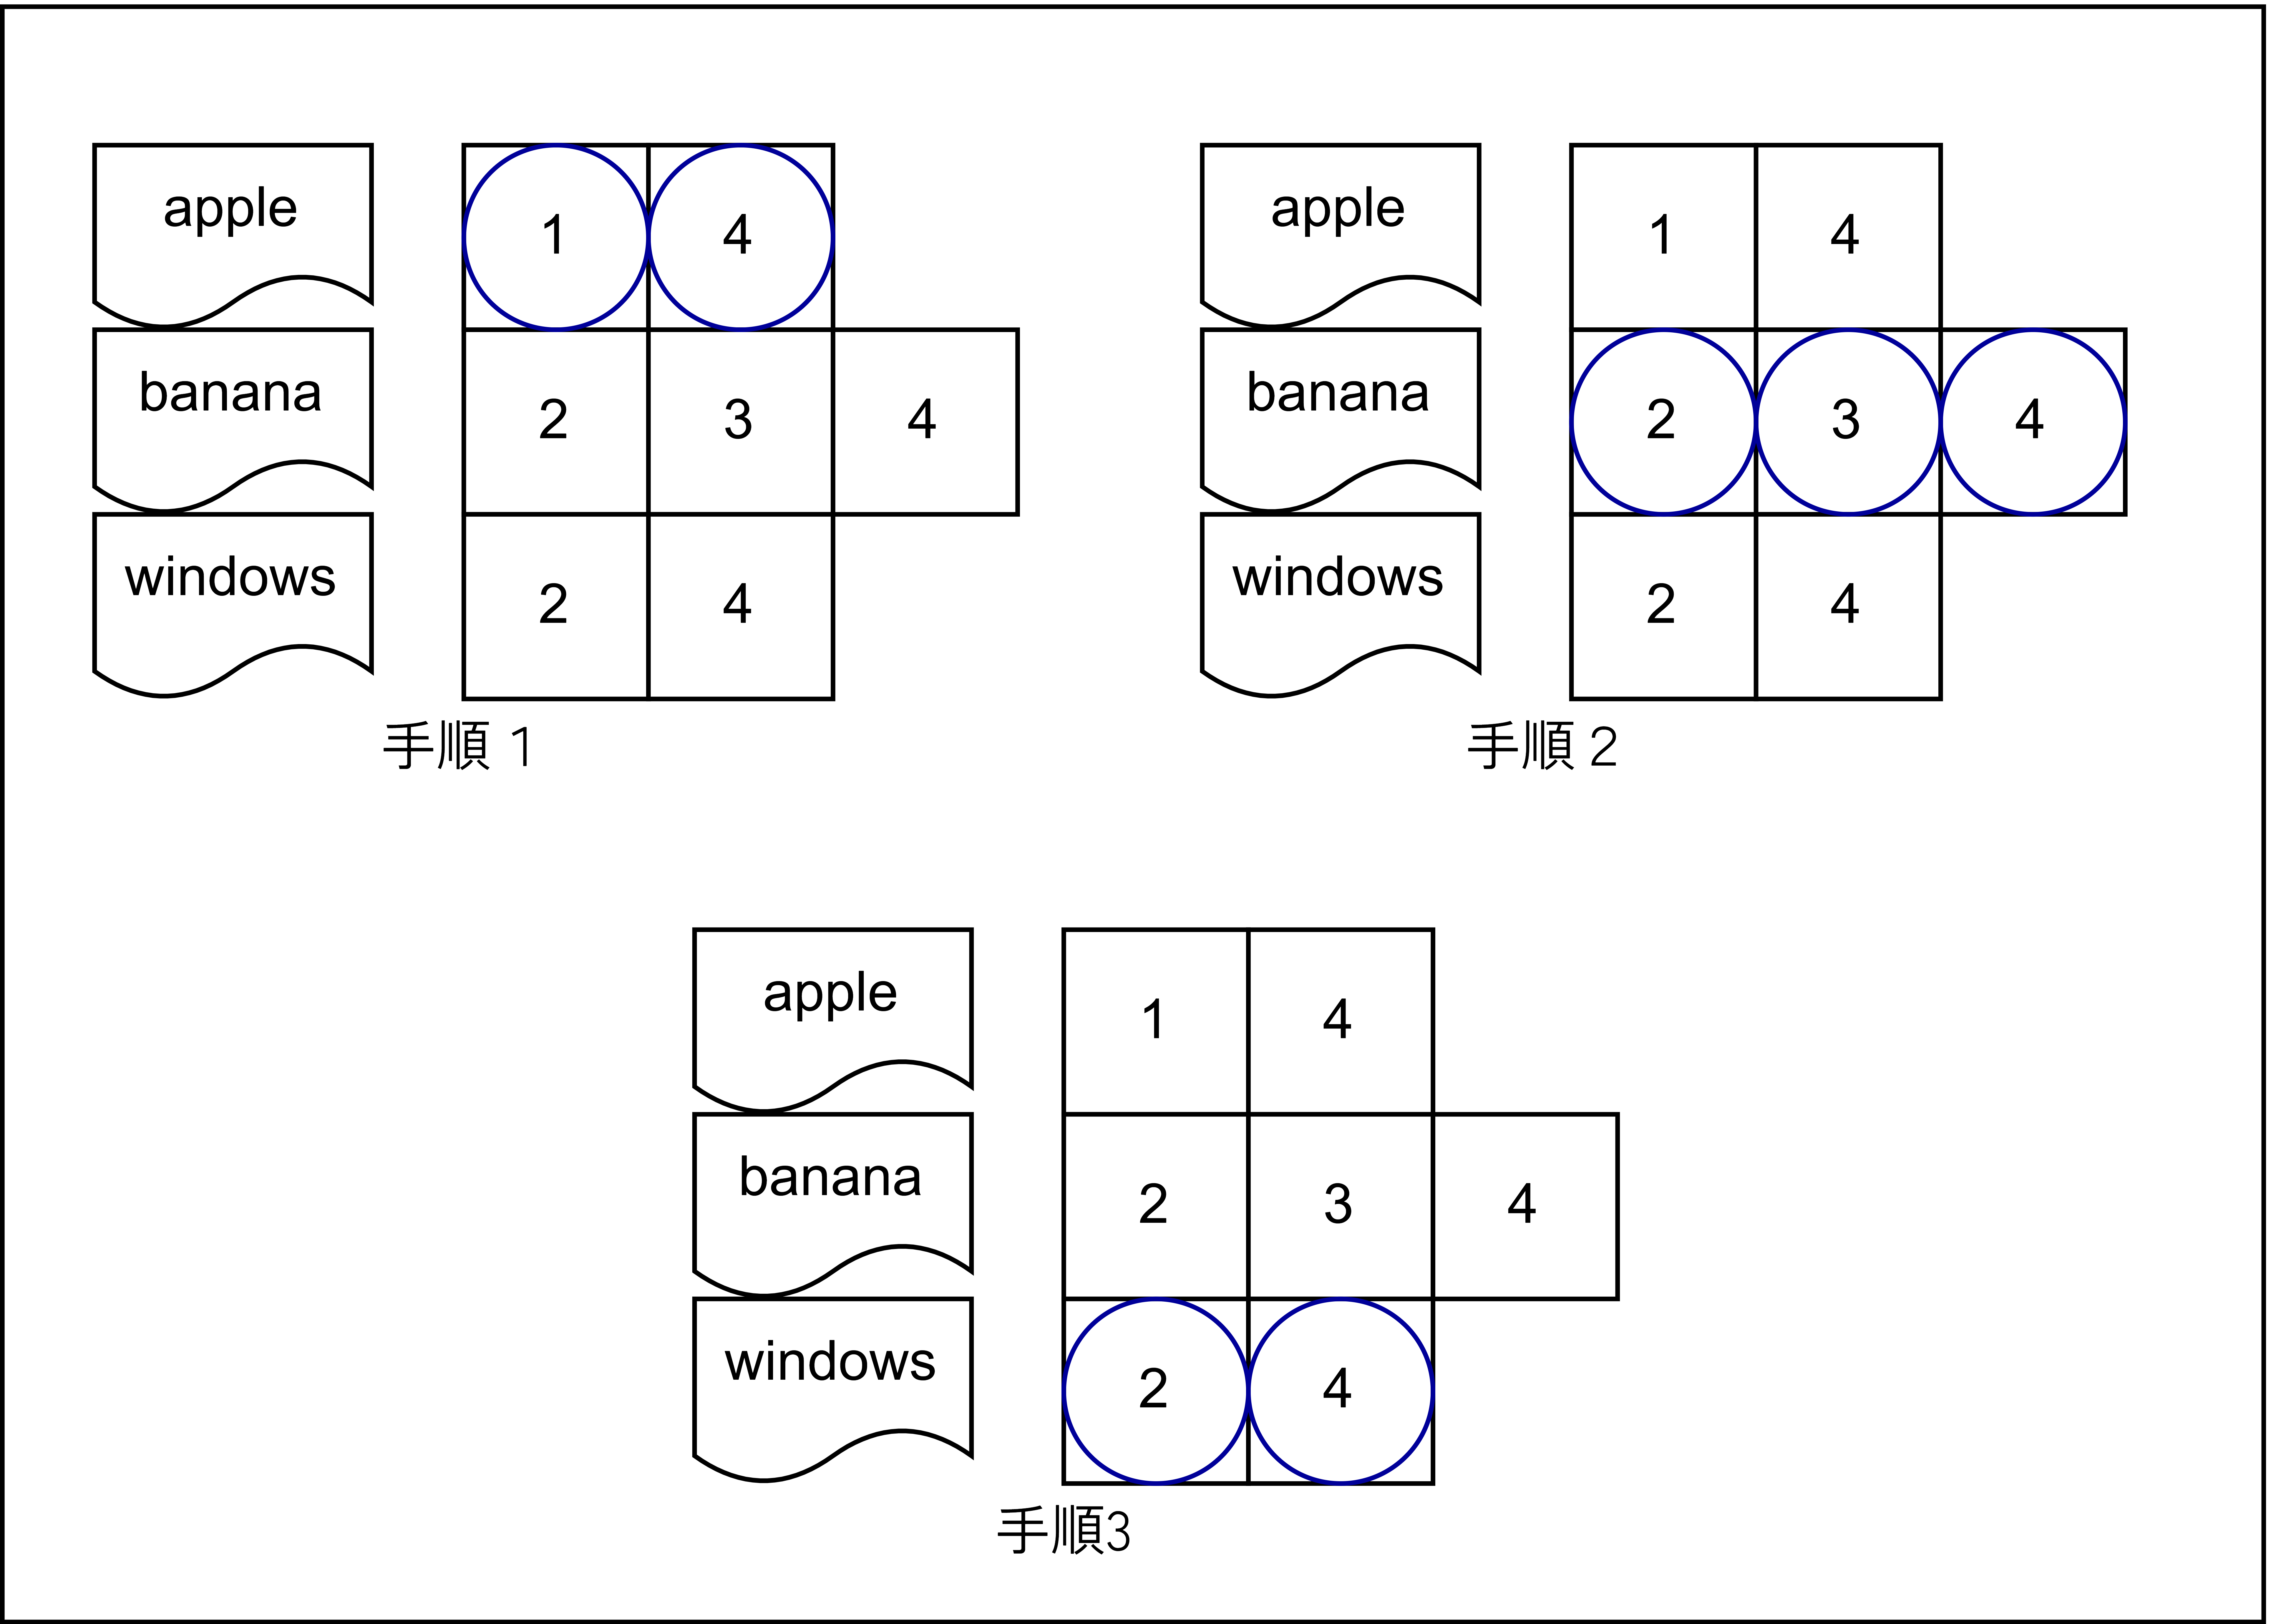
\includegraphics[width=8.7cm]{img/taat.png}
        \caption{TAATの手順}
        \label{fig:TAAT}
    \end{figure}
    
    \item DAAT (Document-At-A-Time)
    \begin{description}
        \setlength{\leftskip}{0.25cm}
        \item {テキスト単位で処理を行う.
        \begin{enumerate}[手順 1]
        \setlength{\leftskip}{0.7cm}
            %\item テキストの投稿時間が最新のテキストが根に来るようなヒープ$H$を用意する.
            \item 最も投稿時間の新しいテキストが根に来るヒープ$H$を用意する.
            \item \label{daat:rep} $u_T$から単語$t_1$を取り出し,対応するリストの先頭を$H$に追加する
            \item 手順\ref{daat:rep}をすべての単語に対して行う.
            \item \label{daat:heap}ヒープ$H$から最も新しいテキストを取り出し,所属するリストの次のテキストを再びヒープ$H$に追加する.
        \end{enumerate}
            TAATとは異なり手順\ref{daat:heap}で新しいテキストから優先してテキストを参照することが出来るため,新しいテキストからマッチング判定をすることが可能である.DAATの手順を図\ref{fig:DAAT}に示す.
        }
        
        \begin{figure}[H]
            \centering
            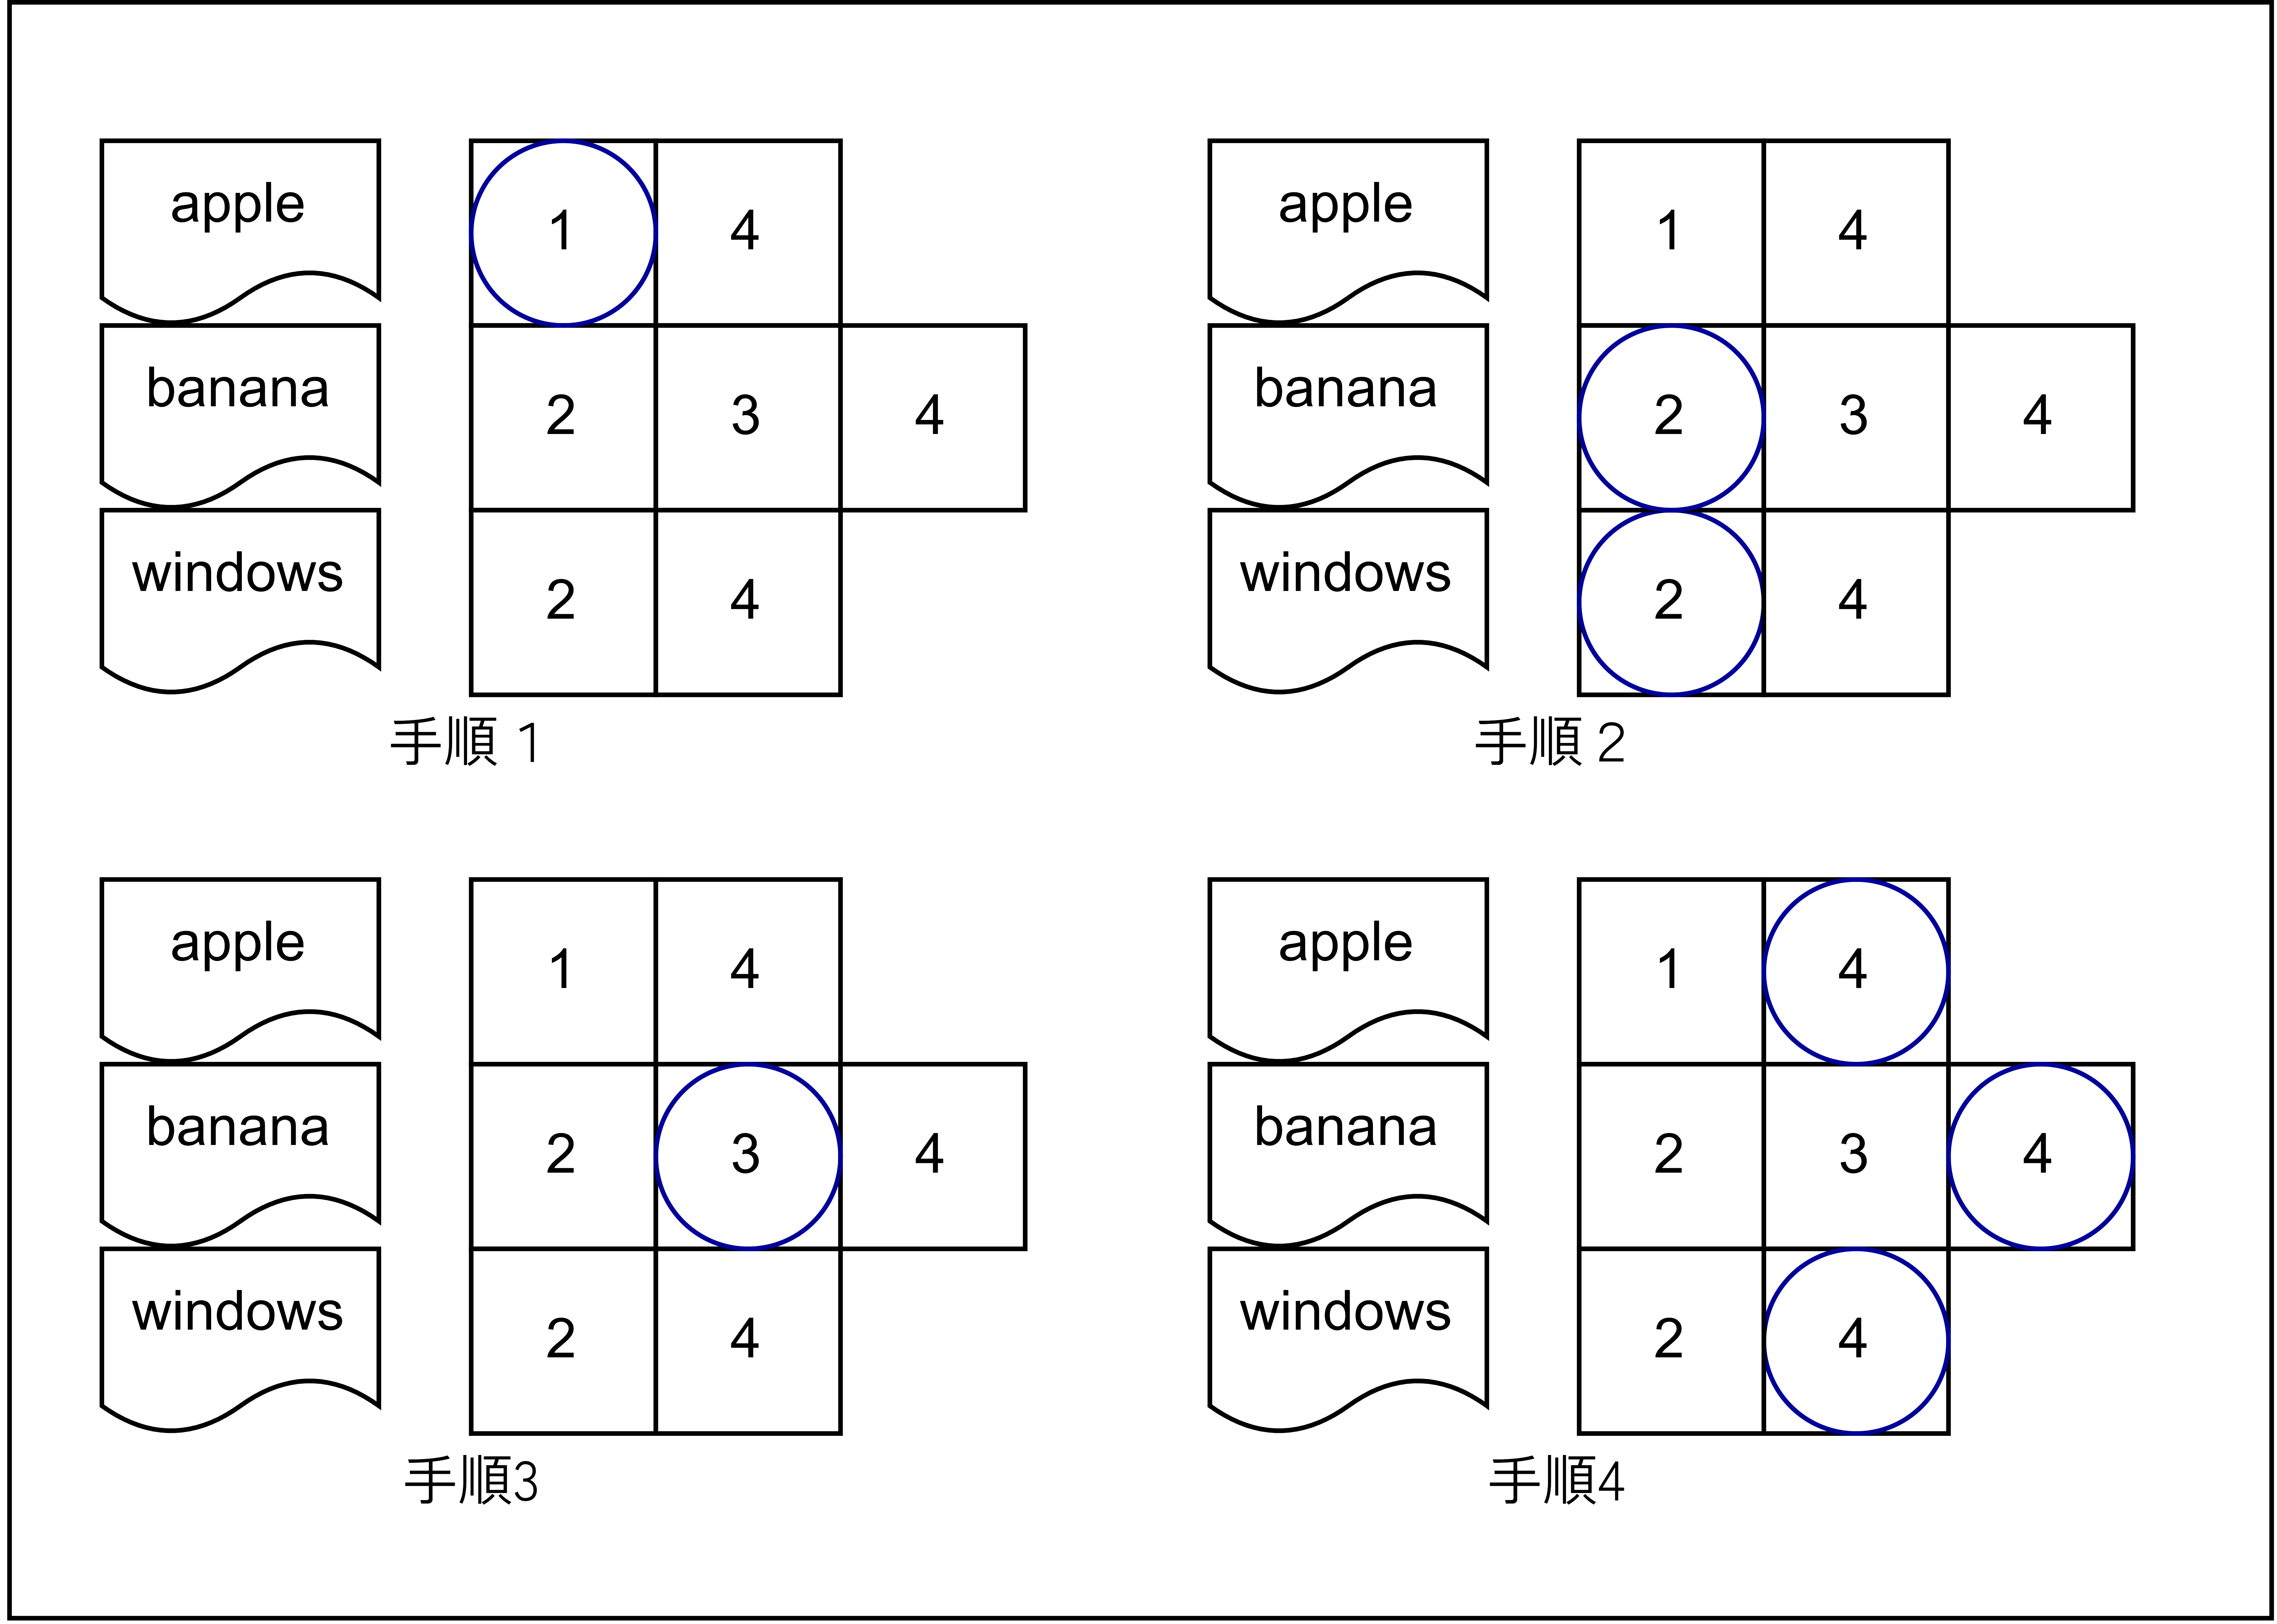
\includegraphics[width=8.7cm]{img/daat.png}
            \caption{DAATの手順}
            \label{fig:DAAT}
        \end{figure}
        
        %\item テキストに存在する単語に対応する集合に対して並列して処理を行う.転置インデクスのリストの中身がIDによって昇順や降順になっているとき,並列してリストの中身を走査することで同一テキストIDごとに処理を行うことができる.
    \end{description}
\end{itemize}
%エリとなるテキストがある場合,そのテキストに存在する単語についてひとつずつ転置インデクスを参照することで,#その単語がどのテキストに含まれているかをIDを通して高速に知ることができる.このとき,転置インデクスを用いた参照方法として主に2つの方法が存在し,その方法を今回の環境を用いて説明する.
